\documentclass[../xlapes02]{subfiles}
\begin{document}
    \chapter{Experiments and Results}\label{sec:experiments-and-results}
    In this chapter


    \section{Weights \& Biases}\label{subsubsec:wandb}
    Weights \& Biases is a machine learning experiment tracking and visualization tool that helps data scientists and machine learning practitioners monitor and manage their experiments. It provides a unified interface for logging and visualizing experiment metrics, hyperparameters, and other relevant information, making it easier to analyze, compare, and reproduce experiments.

    Wandb offers a wide range of features, including:
    \begin{itemize}
        \item Experiment tracking: Wandb allows users to log experiment metrics such as loss, accuracy, and other custom metrics in real-time during training. These metrics are logged to a central dashboard, making it easy to monitor and compare multiple experiments.
        \item Hyperparameter tuning: Wandb supports hyperparameter sweeps, allowing users to explore different hyperparameter configurations in parallel and find optimal hyperparameter settings for their models.
        \item Visualizations: Wandb provides various visualization tools, including interactive plots, histograms, confusion matrices, and more, to help users analyze and understand experiment results.
        \item Artifact management: Wandb allows users to log and version datasets, models, and other artifacts, making it easy to track and reproduce experiments with specific data and model versions.
        \item Collaboration: Wandb enables team collaboration by allowing users to share experiment results, visualizations, and artifacts with team members, facilitating communication and collaboration among team members.
    \end{itemize}

    Agent's traning and testing runs are logged publicly on Wandb Website. The results of each run together with saved models and datasets can be found at~\url{https://wandb.ai/investai/portfolio-allocation}.
    W\&B Api is very reach and offer a lot of features, therefore we will not describe them in this thesis. The documentation can be found at~\url{https://docs.wandb.ai/}.


    \section{The focus of the Study}\label{sec:the-focus-of-the-study}
    TODO


    \section{Metrics Comparison}\label{sec:metrics-comparison}
    TODO

    \subsection{Baselines and Backtesting}\label{subsec:baselines-and-backtesting}
    TODO
%    \begin{figure}[h]
%        \centering
%        \begin{subfigure}[b]{0.3\textwidth}
%            \centering
%            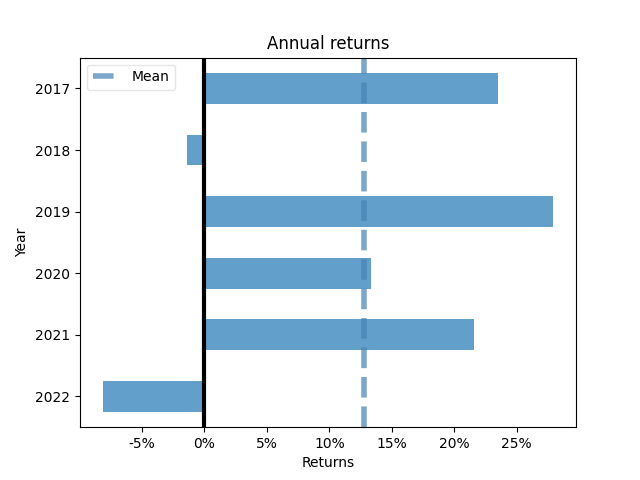
\includegraphics[width=\textwidth]{image/figure/annual_returns_max_model}
%            \caption{$y=x$}
%            \label{fig:y equals x}
%        \end{subfigure}
    %            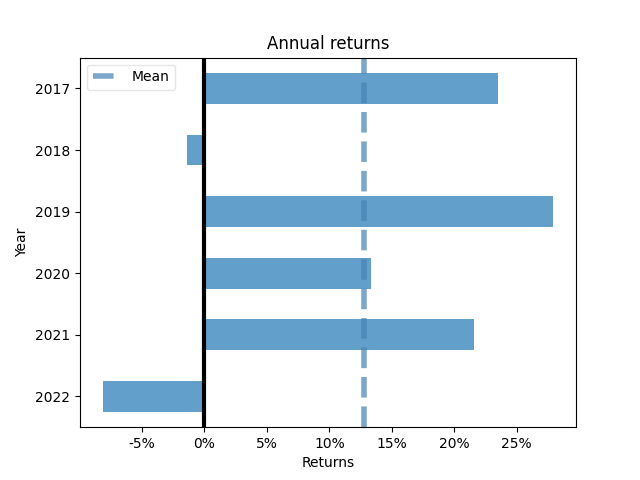
\includegraphics[width=0.8\textwidth]{image/figure/annual_returns_max_model}
%        \hfill
%        \begin{subfigure}{0.45\textwidth}
%            \centering
%%            \includegraphics[width=\linewidth]{image2}
%            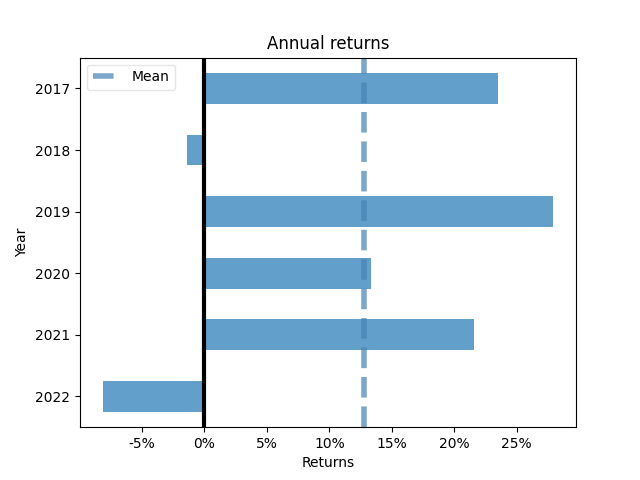
\includegraphics[width=\linewidth]{image/figure/annual_returns_max_model}
%            \caption{Image 2}
%        \end{subfigure}
%
%        \vspace{0.5cm}
%
%        \begin{subfigure}{0.45\textwidth}
%            \centering
%%            \includegraphics[width=\linewidth]{image3}
%            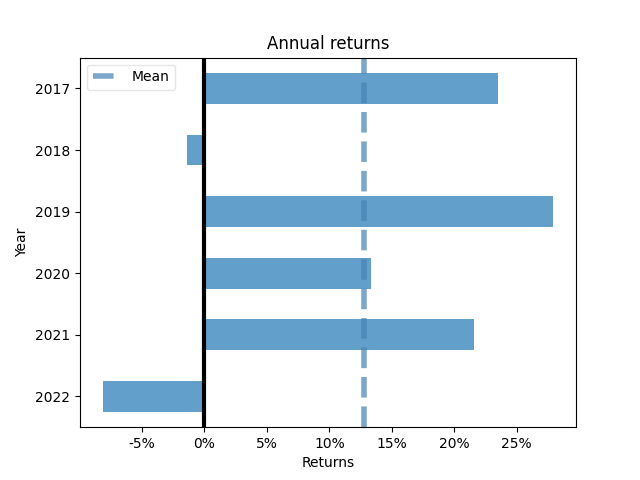
\includegraphics[width=\linewidth]{image/figure/annual_returns_max_model}
%            \caption{Image 3}
%        \end{subfigure}
%        \hfill
%        \begin{subfigure}{0.45\textwidth}
%            \centering
%%            \includegraphics[width=\linewidth]{image4}
%            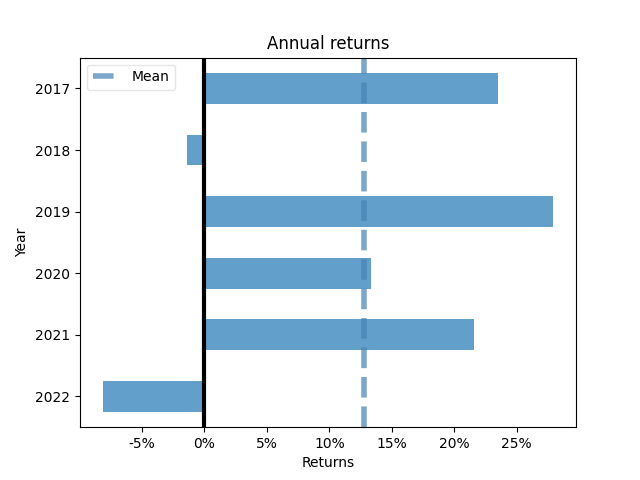
\includegraphics[width=\linewidth]{image/figure/annual_returns_max_model}
%            \caption{Image 4}
%        \end{subfigure}
%        \caption{Four Images in a Grid}
%        \label{fig:four_images}
%    \end{figure}

    \subsection{Reinforcement Learning Algorithms}\label{subsec:rl-algorithms}
    TODO

    \subsection{Hyperparameters}\label{subsec:hyperparameters}
    TODO


    \section{Summary}\label{sec:summary}
    TODO


\end{document}
